\documentclass[a4paper]{article}
\usepackage[utf8]{inputenc}
\usepackage[spanish, es-tabla, es-noshorthands]{babel}
\usepackage[table,xcdraw]{xcolor}
\usepackage[a4paper, footnotesep = 1cm, width=22cm, top=2.5cm, height=25cm, textwidth=20cm, textheight=25cm]{geometry}
%\geometry{showframe}

\usepackage{tikz}
\usepackage{amsmath}
\usepackage{amsfonts}
\usepackage{amssymb}
\usepackage{float}
\usepackage{graphicx}
\usepackage{caption}
\usepackage{subcaption}
\usepackage{multicol}
\usepackage{multirow}
\usepackage{wrapfig}
\setlength{\doublerulesep}{\arrayrulewidth}
\usepackage{booktabs}

\usepackage{hyperref}
\hypersetup{
    colorlinks=true,
    linkcolor=blue,
    filecolor=magenta,      
    urlcolor=blue,
    citecolor=blue,    
}

\newcommand{\note}[1]{
	\begin{center}
		\huge{ \textcolor{red}{#1} }
	\end{center}
}

\setcounter{topnumber}{2}
\setcounter{bottomnumber}{2}
\setcounter{totalnumber}{4}
\renewcommand{\topfraction}{0.85}
\renewcommand{\bottomfraction}{0.85}
\renewcommand{\textfraction}{0.15}
\renewcommand{\floatpagefraction}{0.8}
\renewcommand{\textfraction}{0.1}
\setlength{\floatsep}{5pt plus 2pt minus 2pt}
\setlength{\textfloatsep}{5pt plus 2pt minus 2pt}
\setlength{\intextsep}{5pt plus 2pt minus 2pt}

\newcommand{\quotes}[1]{``#1''}
\usepackage{array}
\newcolumntype{C}[1]{>{\centering\let\newline\\\arraybackslash\hspace{0pt}}m{#1}}
\usepackage[american]{circuitikz}
\usetikzlibrary{calc}
\usepackage{fancyhdr}
\usepackage{units} 

\graphicspath{{../Ejercicio-1/}{../Ejercicio-2/}{../Ejercicio-3/}{../Ejercicio-4/}{../ParteI/}{../ParteII/}{../ParteIII/}{../ParteIV/}}

\pagestyle{fancy}
\fancyhf{}
\lhead{22.14 - Electrónica IV}
\rhead{Mechoulam, Lambertucci, Londero}
\rfoot{Página \thepage}


\begin{document}

\subsection{Diferencias Switch Ideal - MOS}
En esta sección se reemplaza la llave ideal por un MOSFET con un circuito de disparo igual al del primer ejercicio. Realizando los mismo análisis se obtienen los siguientes gráficos:

\begin{multicols}{2}
\begin{figure}[H]
	\centering
	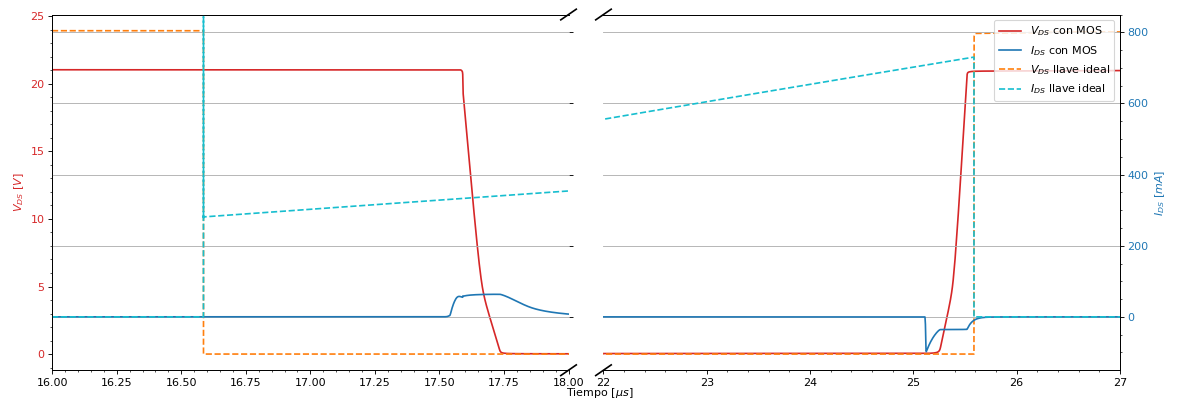
\includegraphics[width=\linewidth]{ImagenesEjercicio-3/ids-vds-2v3}
	\caption{Conmutaciones $V_{DS}$ e  $I_{DS}$.}
	\label{fig:ej3:conmutacionON_OFF_VDS_IDS}
\end{figure}
\begin{figure}[H]
	\centering
	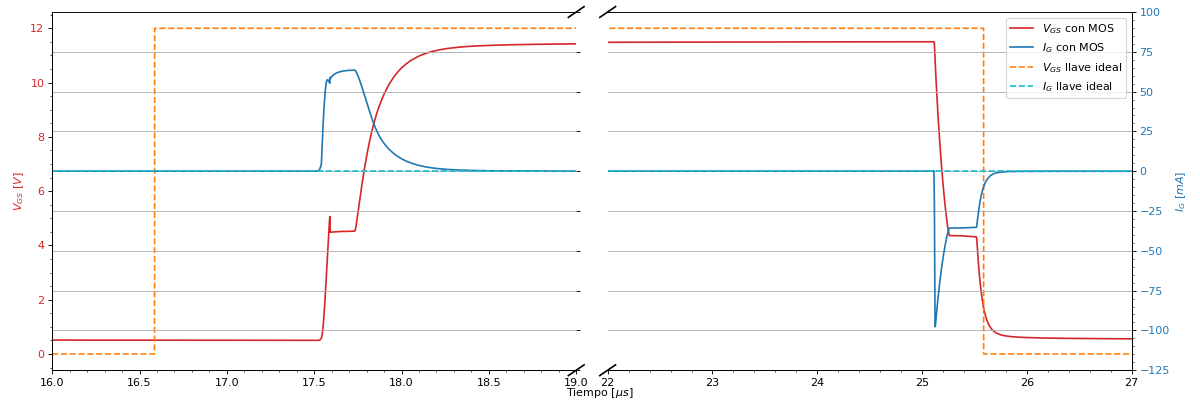
\includegraphics[width=\linewidth]{ImagenesEjercicio-3/ig-vgs-2v3}
	\caption{Conmutaciones $V_{GS}$ e  $I_{G}$.}
	\label{fig:ej3:conmutacionON_OFF_VGS_IG}
\end{figure}
\end{multicols}
\begin{multicols}{2}
\begin{figure}[H]
	\centering
	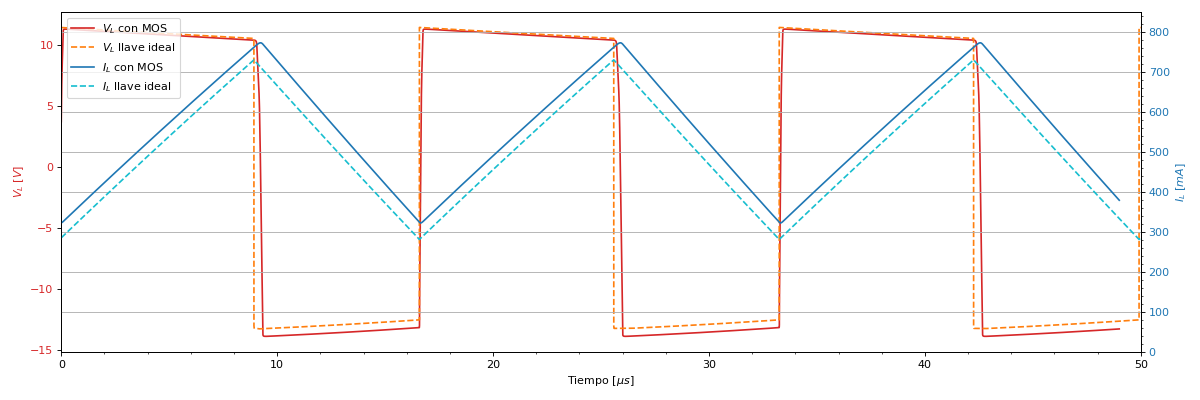
\includegraphics[width=\linewidth]{ImagenesEjercicio-3/il-vl-2v3}
	\caption{Tensión y Corriente sobre la bobina.}
	\label{fig:ej3:Il_Vl}
\end{figure}
\begin{figure}[H]
	\centering
	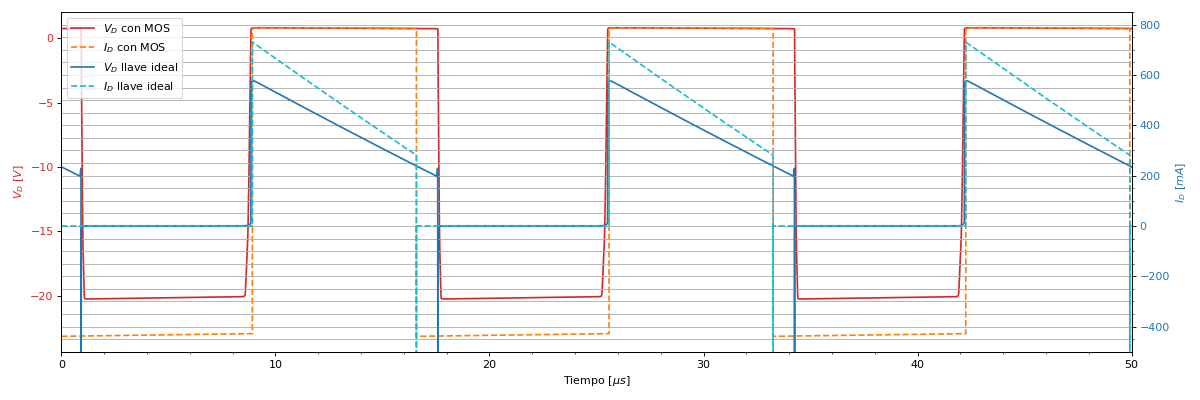
\includegraphics[width=\linewidth]{ImagenesEjercicio-3/id-vd-2v3}
	\caption{Tensión y Corriente sobre el diodo.}
	\label{fig:ej3:Id_Vd}
\end{figure}
\end{multicols}

Con el cambio mencionado, se pueden notar variaciones en la $V_L$ y en el duty cycle, el cual aumentó respecto al que se daba con un switch ideal. La variación porcentual de esta variable es $\Delta DC = 0.95 \% $. También se observa la diferencia en los tiempos de conmutación, la cual se debe a que en la llave ideal los cambios son instantáneos mientras que con la real no lo es. Con respecto a la diferencia de offset en la corriente, la causa se debe a la $r_{DS}$ existente en el MOSFET y no en la llave. Por último se puede observar que la corriente de reverse recovery del diodo ahora se ve acotada a $I_{rr}\approx 2.8 \ A$, la cual es menor a la registrada en el caso anterior.


\subsection{Potencia}
Se verá la potencia disispada en el MOS debido a la conmutación en cada período.
Para la conmutaciónde off será la siguiente:
\begin{equation}
P_{MOS-off}=I_o \cdot V_o \cdot t_{conm} \cdot f_{sw} = 105.06mW
\end{equation}
Donde $I_o=570mA \ \ \ V_o = 24V \ \ \ t_{conm}= 128ns \ \ \ f_{sw}=60KHz$ 
Para la conmutación On será:
\begin{equation}
P_{MOS-on}=I_o \cdot V_o \cdot t_{conm} \cdot f_{sw} = 0.41W
\end{equation}
Donde $I_o=570mA+1.7A \ \ \ V_o = 24V \ \ \ t_{conm}= 128ns \ \ \ f_{sw}=60KHz$ . \\
Mientras que en la fuente entregará
$P_{V_2}=I_o \cdot V_2 = 6.84W$
Esta potencia es un $7.5 \%$ de la potencia entregada por $V_2$
\subsection{Tiempos de Conmutación}
Los tiempos de conmutación se ven alterados respecto al circuito de la primera sección, ya que los valores de $V_{GS-IO}$, $I_{G-IO}$ e $I_{DS}$ dependen principalmente del circuito de aplicación. Dada la topología del circuito (Boost), cuando el MOSFET se encuentra apagado, el circuito se simplifica un RLC. Cuando se encuentra prendido se presentan dos circuitos: un RL del lado del generador y un RC en la carga. Es importante remarcar esto ya que esto afecta los tiempos $t_{ri}$ ,$t_{fv}$, $t_{d_{off}}$, $t_{rv}$ y  $t_{fi}$. Para el caso de disparo con MOSFET son los siguientes:
\begin{table}[H]
\center
\begin{tabular}{cccccc}
\hline
$t_{on}$ & $t_{ri}$ & $t_{fv}$ & $t_{doff}$ & $t_{rv}$ & $t_{fi}$          \\	\hline
45 ns       & 15 ns       & 158 ns      & 145 ns        & 128 ns      & 10 ns     \\	 	\hline
\end{tabular}
\caption{Tiempos de conmutación en el disparo del MOSFET.}
\end{table}

Algo a notar en las Figuras (\ref{fig:ej3:Id_Vd_SWITCH_BOOST}) y (\ref{fig:ej3:Il_Vl_SWITCH_BOOST}) es que la corriente por la bobina y el diodo, al igual que la tensión sobre los mismos, depende de la carga. Es por este motivo es razonable que sus valores sean distintos. En cuanto a la corriente de recovery se puede ver que con un MOSFET toma un valor razonable a diferencia del uso de un componente ideal. 
\begin{multicols}{2}
\begin{figure}[H]
	\centering
	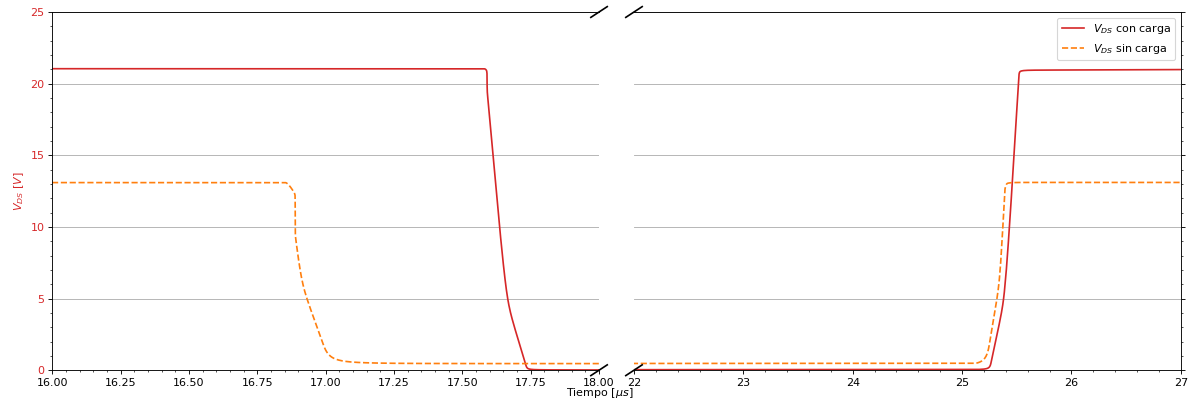
\includegraphics[width=\linewidth]{ImagenesEjercicio-3/ids-vds-1v3}
	\caption{Conmutaciones $V_{DS}$ e  $I_{DS}$ llave con y sin Boost.}
	\label{fig:ej3:conmutacionON_OFF_VDS_IDS_SWITCH_BOOST}
\end{figure}
\begin{figure}[H]
	\centering
	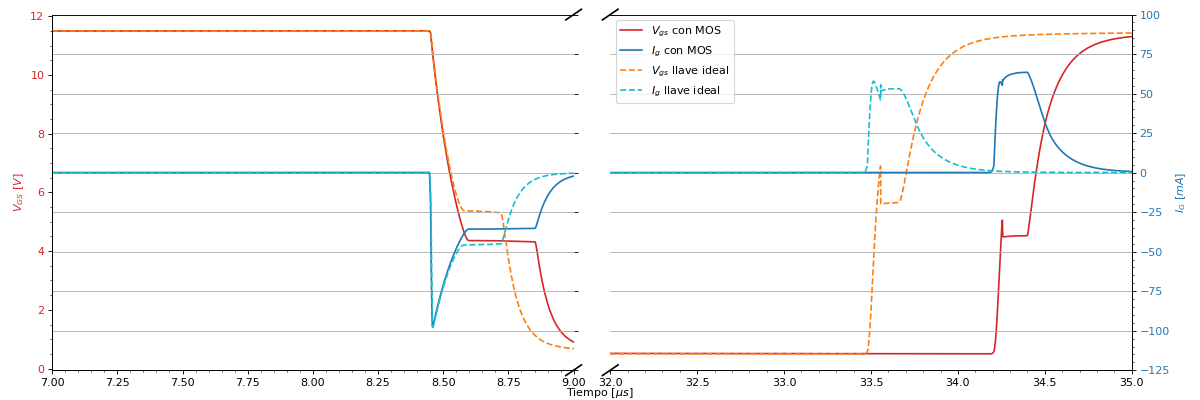
\includegraphics[width=\linewidth]{ImagenesEjercicio-3/ig-vgs-1v3}
	\caption{Conmutaciones $V_{GS}$ e  $I_{S}$ llave con y sin Boost.}
	\label{fig:ej3:conmutacionON_OFF_VGS_IG_SWITCH_BOOST}
\end{figure}
\end{multicols}
\begin{multicols}{2}
\begin{figure}[H]
	\centering
	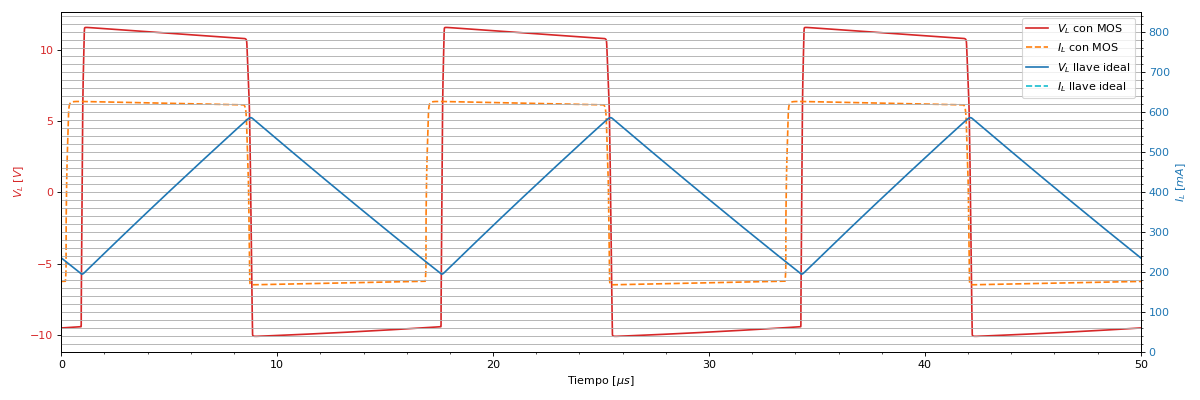
\includegraphics[width=\linewidth]{ImagenesEjercicio-3/il-vl-1v3}
	\caption{Tensión y Corriente sobre la bobina llave con y sin Boost.}
	\label{fig:ej3:Il_Vl_SWITCH_BOOST}
\end{figure}
\begin{figure}[H]
	\centering
	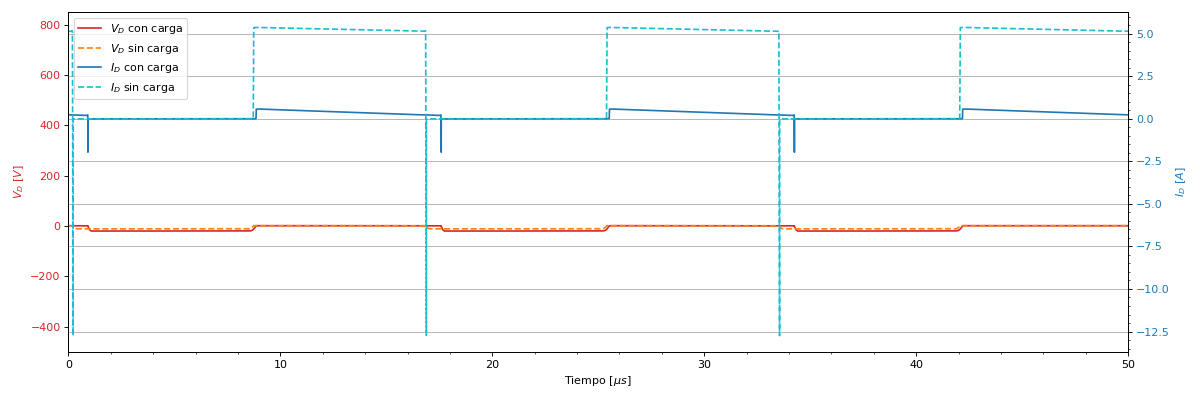
\includegraphics[width=\linewidth]{ImagenesEjercicio-3/id-vd-1v3}
	\caption{Tensión y Corriente sobre el diodo llave con y sin Boost.}
	\label{fig:ej3:Id_Vd_SWITCH_BOOST}
\end{figure}
\end{multicols}

\end{document}